\documentclass{article}
\usepackage[margin=3cm]{geometry}
\usepackage{float}
\usepackage{graphicx}
\usepackage{amsmath}
\usepackage{soul}

\title{Evolución de Redes de Flujo Adaptativas}
\author{}
\date{}

\begin{document}

\maketitle

\section{Introducción}

En este proyecto estudiamos la evolución de una red de flujo adaptativa que modela sistemas biológicos. El objetivo es comprender cómo emergen estructuras optimizadas a partir de reglas locales simples.

\section{Sistema}

Estudiamos la evolución de una red de flujo adaptativa. Desde las puntas del árbol ingresa un fluido que es transportado hacia el nodo inicial o sumidero, por donde el fluido deja el sistema.

El modelo tratado acá es una simplificación puramente topológica, la red no está sometida a las restricciones del espacio. Por lo mismo, el sistema está siempre en su mínimo topológico, los nodos se encuentran siempre en una bifurcación.

Por simplicidad, los únicos nodos que pueden realizar acciones son las puntas, es decir, los nodos de conectividad 1 excepto el sumidero. Estas puntas pueden:

\begin{itemize}
    \item Retraerse ($l_{ij}$ se reduce de $l_0 \eta (t)$, si baja de 0 el nodo desaparece) con probabilidad $p_0$
    \item Crecer ($l_{ij}$ crece de $l_0\eta (t)$) con probabilidad $p_1$
    \item Bifurcarse (nacen 2 nodos/ductos nuevos) con probabilidad $p_2$
\end{itemize} 

\section{Modelos más simples}

\subsection{Modelo Probabilístico}

Para comenzar, desarrollamos un modelo puramente probabilístico: Las tres probabilidades son constantes. La punta que actúa es elegida aleatoriamente.

La evolución del árbol (y su supervivencia) dependen completamente de la relación entre las probabilidades (Fig. \ref{fig:evolucion_tamano_proba}). 

\begin{figure}[h!]
    \centering
    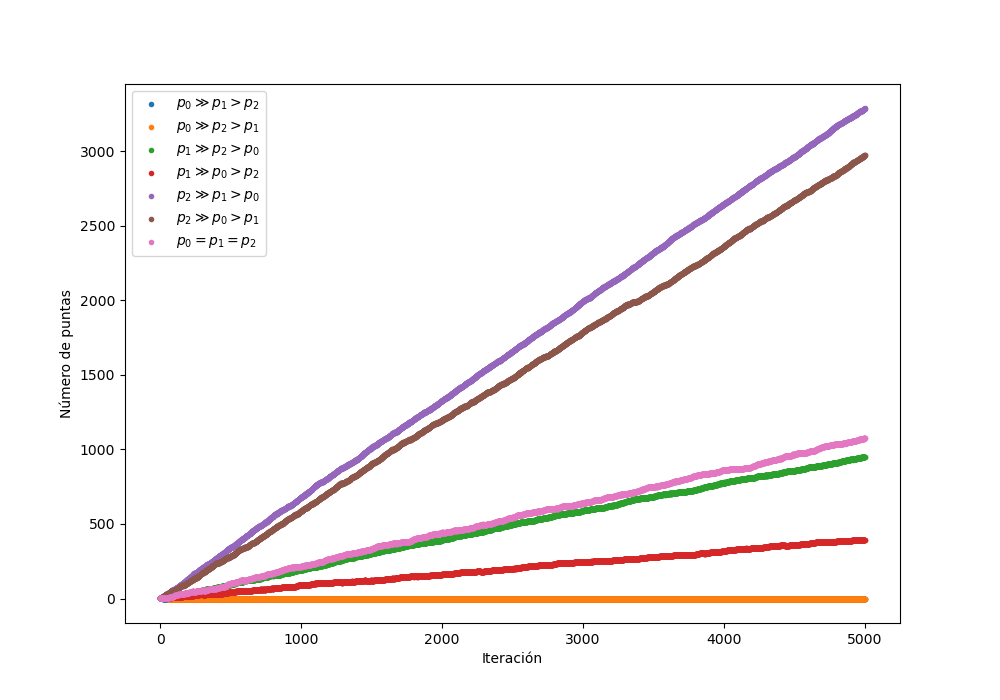
\includegraphics[width=0.8\textwidth]{graficos_proba/N(t)_comparado.png}
    \caption{Evolución temporal del tamaño del árbol.}
    \label{fig:evolucion_tamano_proba}
\end{figure}

Vemos que si la retracción domina, el sistema muere casi inmediatamente. Mientras que si domina una de las otras, el crecimiento es siempre lineal respecto a la iteración.

\subsection{Optimización y flujo}

Anteriormente, el flujo no tenía ningún efecto sobre el sistema. Ahora, este debe optimizarse para minimizar la perdida de energía y mantener un volumen constante, dado por $\mathcal{K}$.

Entonces, cada ducto $ij$ tiene asociada una conductancia: $C_{ij} = \frac{\pi r_{ij}^4}{8\mu l_{ij}}$. Calculamos también el flujo del fluido $Q_{ij}$ en cada ducto propagando el flujo entrante de las puntas. Entonces, la conductancia óptima es:

$$ C_{ij}^* = \frac{\langle Q_{ij}(t)^2\rangle_T^{2/3} \mathcal{K}}{\left( \sum_{<ij>} \langle Q_{ij}(t)^2\rangle_T^{1/3} l_{ij}\right)^2 l_{ij}} $$

En cada iteración, optimizamos las conductancias de toda la red.

Estudiamos el decaimiento de la conductancia promedio de las puntas con $\mathcal{K}=100$, $p_0 = 0.1$, $p_1 = 0.7$, $p_2 = 0.2$ (Fig. \ref{fig:evolucion_conductancia_proba}).

\begin{figure}[h!]
    \centering
    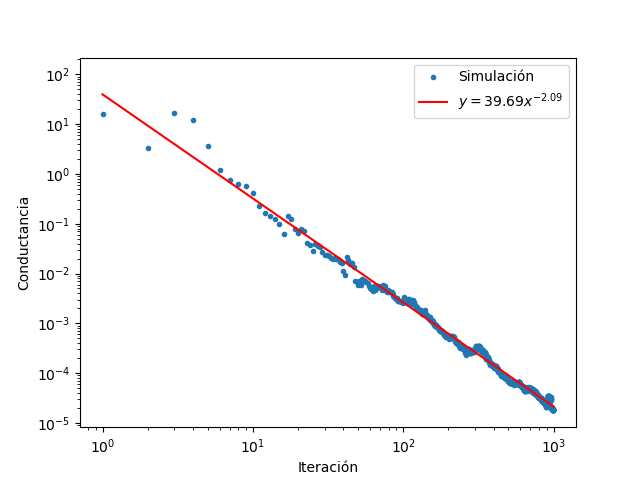
\includegraphics[width=0.8\textwidth]{graficos_proba/Cij_vs_tiempo.png}
    \caption{Evolución temporal de la conductancia.}
    \label{fig:evolucion_conductancia_proba}
\end{figure}

Vemos que esta decae aproximadamente como el inverso del cuadrado de la iteración.

Para encontrarlo analíticamente, podemos hacer algunas aproximaciones suponiendo una evolución homogénea: El largo de todos los ductos es similar, llamémoslo $l$ y el árbol es relativamente simétrico. Además, puesto que el flujo se promedia en el tiempo, en las puntas este es básicamente $q_0$.

Entonces, si $N$ es la cantidad de puntas, el flujo total en cada "nivel" del árbol es $Nq_0$, y hay $\log_2(N)+1$ niveles, por lo que podemos escribir $\left( \sum_{<ij>} \langle Q_{ij}(t)^2\rangle_T^{1/3} l_{ij}\right)^2 l_{ij} \simeq N^{2}\log_2^{2}(N)q_0^{4/3}l^{3}$

Por lo tanto, podemos escribir la conductancia óptima de las puntas como:

$$ C_p \simeq \dfrac{\mathcal{K} \ln^2(2)}{N^{2}\ln^{2}(N)l^{3}} $$

Luego, vimos anteriormente que en el modelo probabilístico, $N \propto i$ (iteración), por lo tanto:

$$ C_p \propto \frac{1}{i^2 \ln^2(i)} $$

\textbf{Discrepancia}: Esto difiere de lo observado en las simulaciones ($1/i^2$), posiblemente debido a que las aproximaciones de homogeneidad y simetría no se cumplen exactamente en el sistema simulado.

\section{Modelo "instantáneo"}

En este modelo las adaptaciones (de conductancia o largo) ocurren instantáneamente. Suponemos que el tiempo que demora en evolucionar el sistema es mucho menor al tiempo entre iteraciones.

\subsection{Probabilidades dependientes de la conductancia}

Ahora introducimos las leyes de crecimiento que nos interesan. La probabilidad de cada acción depende del estado del sistema:

\begin{itemize}
    \item $p_0(C_{ij}) = e^{-C_{ij}/\bar{C}}$
    \item $p_1(C_{ij}) = p_2(C_{ij}) = \dfrac{1 - e^{-C_{ij}/\bar{C}}}{2}$
\end{itemize}

Introducimos una conductancia crítica $\bar{C}$, generalmente pequeña. De esta forma, un ducto con alta conductancia tiende a crecer o bifurcarse, mientras que uno con baja conductancia se retrae. Por cómo se calcula la conductancia óptima, un ducto con alto flujo tiende a crecer, o "explorar", pero está limitado por su largo que disminuye la conductancia.

\subsection{Tiempo de Gillespie}

Hablamos de probabilidades ya que suman 1, pero ahora nos interesa más ver $p_0$, $p_1$ y $p_2$ como tasas en el tiempo. Por lo tanto, es necesario re-escalar el tiempo según el algoritmo de Gillespie. Este aproxima el tiempo transcurrido entre cada iteración dada la tasa a la que ocurren los diferentes eventos:

$$ \tau = \frac{-\ln(r)}{\sum_{<ij>}p_0(C_{ij}) + p_1(C_{ij}) + p_2(C_{ij})} = \frac{-\ln(r)}{N}$$

Donde $r$ es un número aleatorio en $(0,1]$.

\subsection{Elección del nodo}

Hasta ahora, la elección del nodo se realizaba aleatoriamente y luego se escogía la acción según las probabilidades. Sin embargo, puesto que las probabilidades son diferentes para cada punta, tiene más sentido combinar estas dos elecciones para así elegir el evento \{nodo, acción\} más probable.

Por lo tanto, en cada iteración se generan todas las probabilidades de todas las puntas, y luego se elige entre estas de acuerdo a las probabilidades.

\subsection{Evolución temporal}

Con la aplicación de las probabilidades variables aparecen dos fases en la evolución. La primera, muy corta, es una fase de "exploración". La probabilidad de retracción es casi nula ya que la conductancia es mucho mayor a la crítica. El crecimiento hace disminuir las conductancias de las puntas: son los ductos con menos flujo, por lo que se les asigna una conductancia más baja para mantener el volumen. Cuando la conductancia se acerca al valor crítico, la probabilidad de retracción crece. Aquí el sistema entra en una segunda fase, esta estacionaria. Las características del sistema se estabilizan con cierto ruido.

Para las figuras, tomamos como ejemplo un sistema con $K = 1000$ y $\bar{C} = 5\cdot10^{-3}$.

\begin{figure}[h!]
\begin{minipage}{0.5\textwidth}
    \centering
    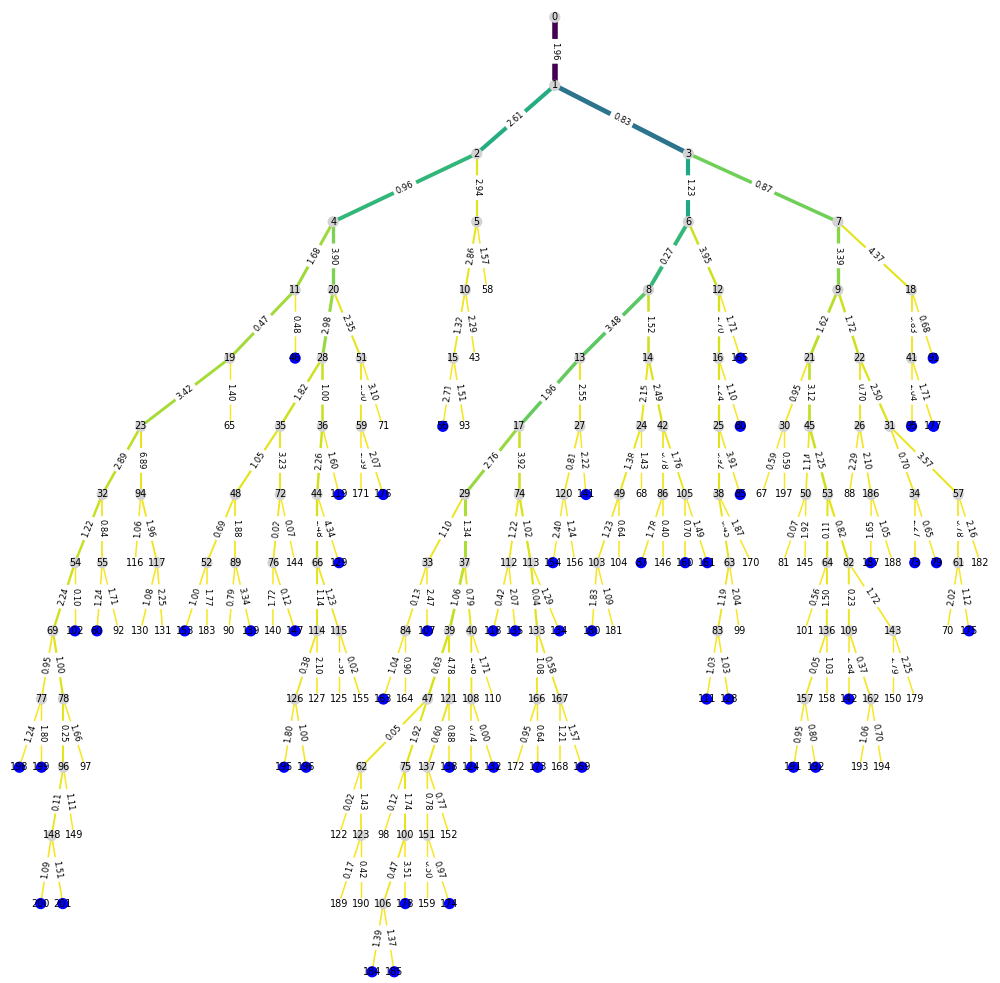
\includegraphics[width=\textwidth]{graficos_inst/arbol_exp.png}
    \caption[]{Árbol en fase de exploración ($t=71$)}
    \label{fig:arbol_exp}
\end{minipage} 
\begin{minipage}{0.5\textwidth}
    \centering
    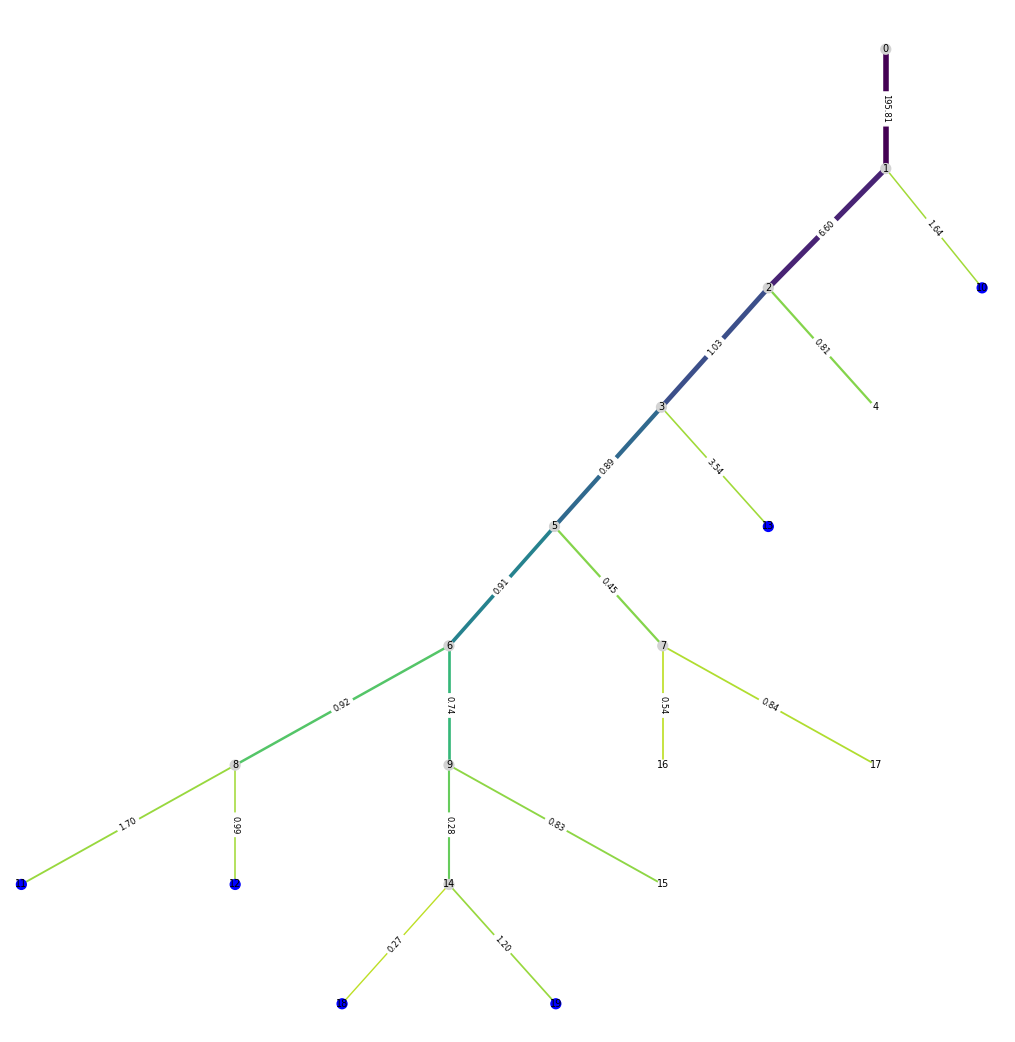
\includegraphics[width=\textwidth]{graficos_inst/arbol_est.png}
    \caption[]{Árbol en fase de estacionaria ($t=3924$)}
    \label{fig:arbol_est}
\end{minipage}   
\end{figure}

\begin{figure}[h!]
    \centering
    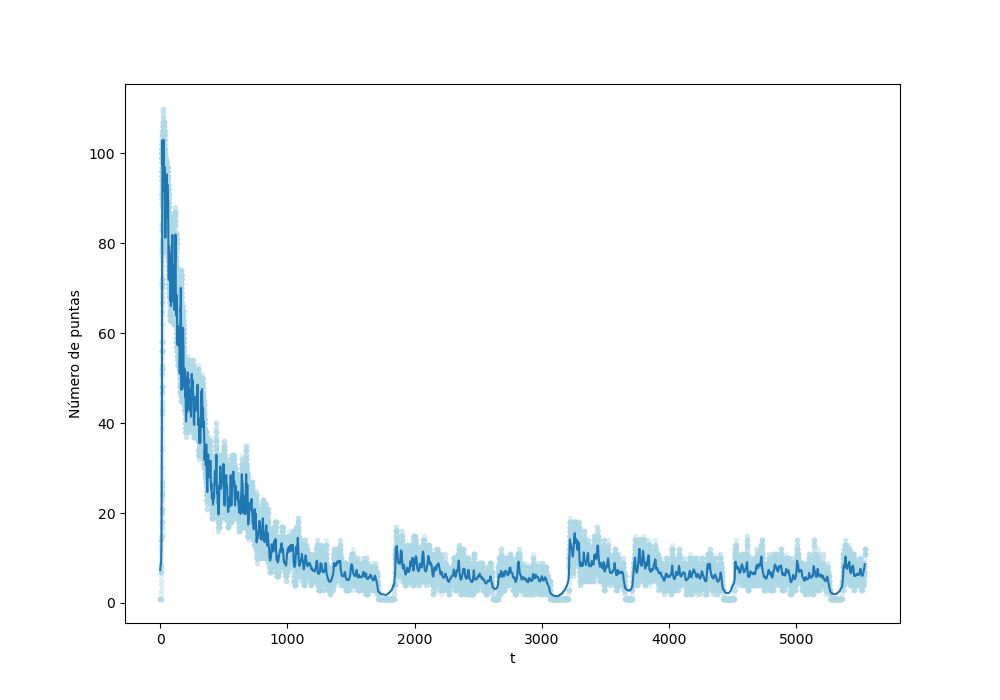
\includegraphics[width=0.8\textwidth]{graficos_inst/N_vs_tiempo.png}
    \caption[]{Evolución temporal de la cantidad de puntas.\footnotemark}
    \label{fig:evolucion_N}
\end{figure}
\footnotetext{La cantidad total de nodos es simplemente el doble.}

\begin{figure}[h!]
    \centering
    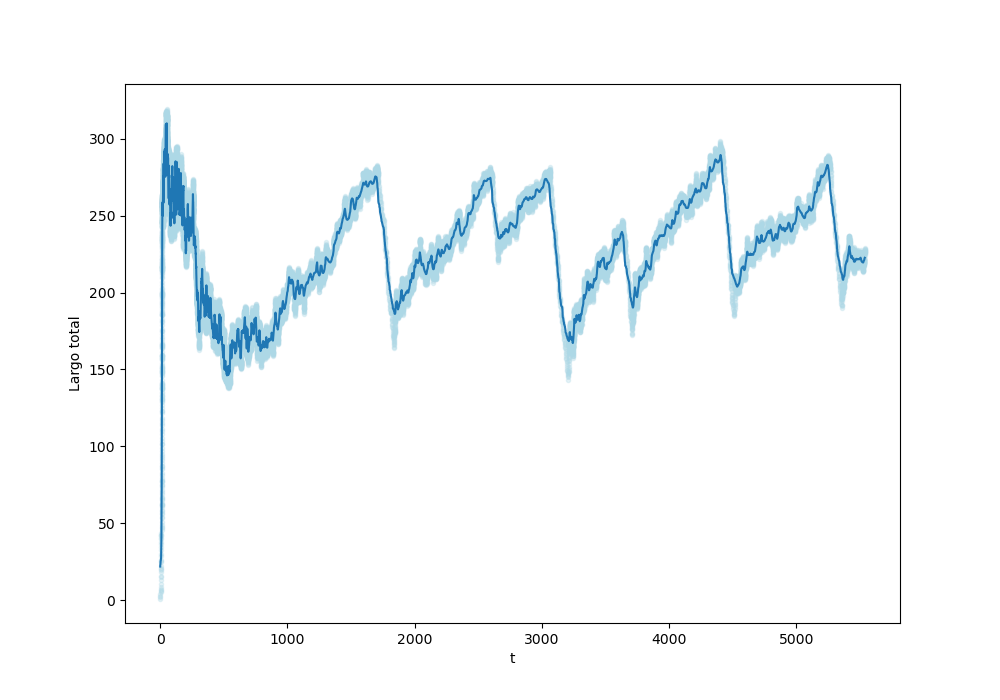
\includegraphics[width=0.8\textwidth]{graficos_inst/largo_vs_tiempo.png}
    \caption{Evolución temporal del largo total del árbol.}
    \label{fig:evolucion_tamano}
\end{figure}

La evolución de las probabilidades refleja las fases, mostrando la dominancia de una u otra acción.

\begin{figure}[h!]
    \centering
    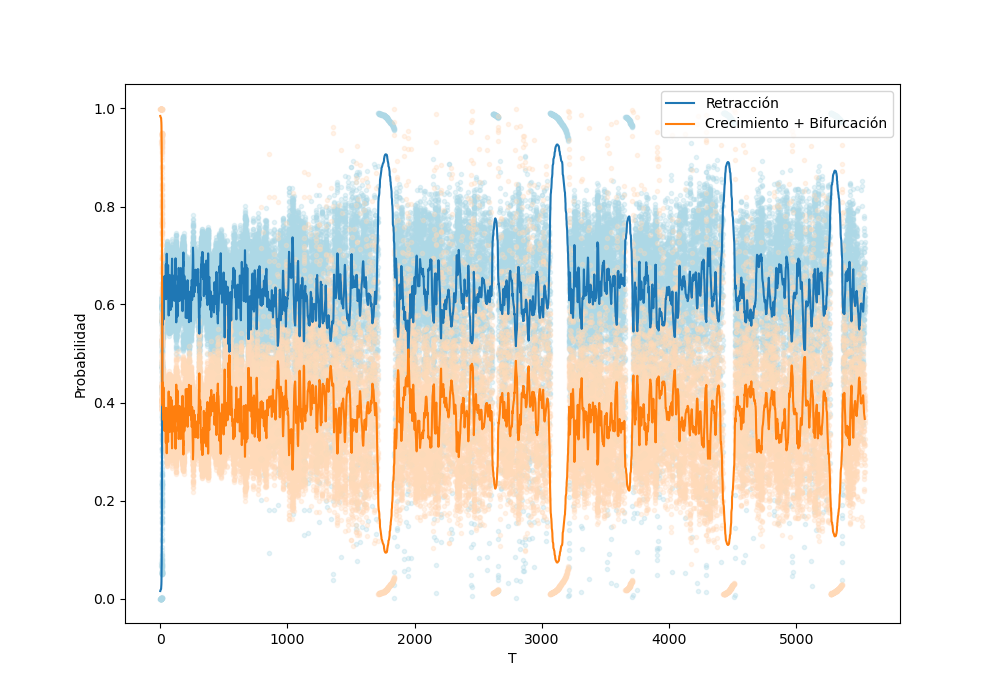
\includegraphics[width=0.8\textwidth]{graficos_inst/probs_vs_tiempo.png}
    \caption{Evolución temporal de las probabilidades promedio.}
    \label{fig:evolucion_probabilidades}
\end{figure}

Finalmente, la conductancia promedio de las puntas converge con el tiempo hacia la conductancia crítica.

\begin{figure}[h!]
    \centering
    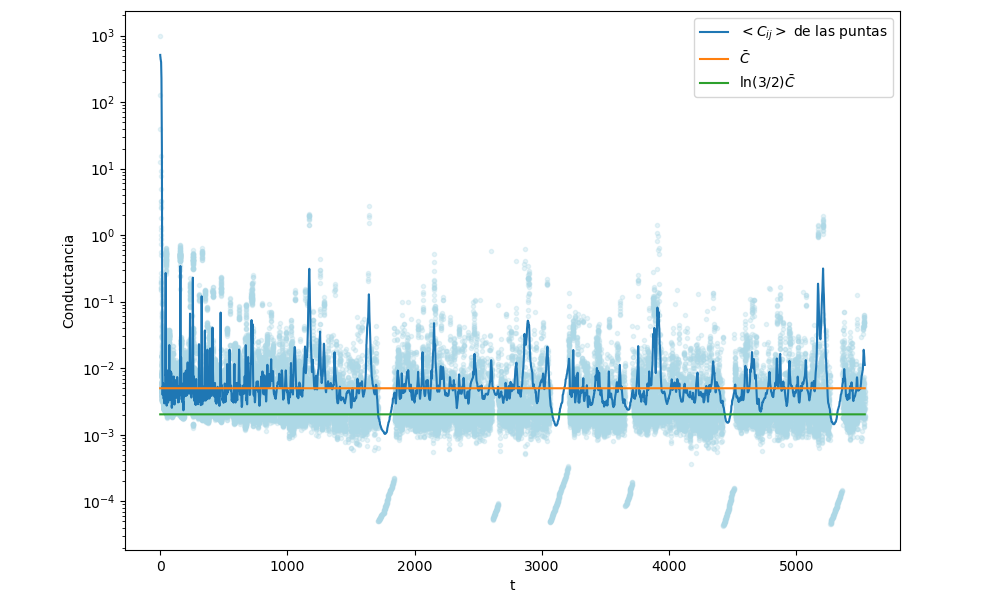
\includegraphics[width=0.8\textwidth]{graficos_inst/Cij_vs_tiempo.png}
    \caption{Evolución temporal de la conductancia.}
    \label{fig:evolucion_conductancia}
\end{figure}

Todos los gráficos tienen unos peaks comunes, que corresponden a fuertes retracciones del árbol. Estos ocurren cuando el primer ducto (o uno de los más antiguos) se vuelve una punta debido a retracciones previas. Al tener un largo considerable, su conductancia es muy baja, lo que aumenta drásticamente su probabilidad de retracción ($p_0 \approx 1$). El ducto se retrae hasta alcanzar una conductancia mayor, momento en que se bifurca en dos pequeños ductos con alta conductancia, causando los picos observados en conductancia promedio y probabilidad de crecimiento.
\newpage
\subsection{Tamaño máximo}

Veamos primero cómo varía el tamaño máximo del árbol con los parámetros. Rápidamente encontramos una relación muy clara entre el tamaño máximo y la razón $\frac{K}{\bar{C}}$ (Fig. \ref{fig:max_vs_KC}).

\begin{figure}[h!]
    \centering
    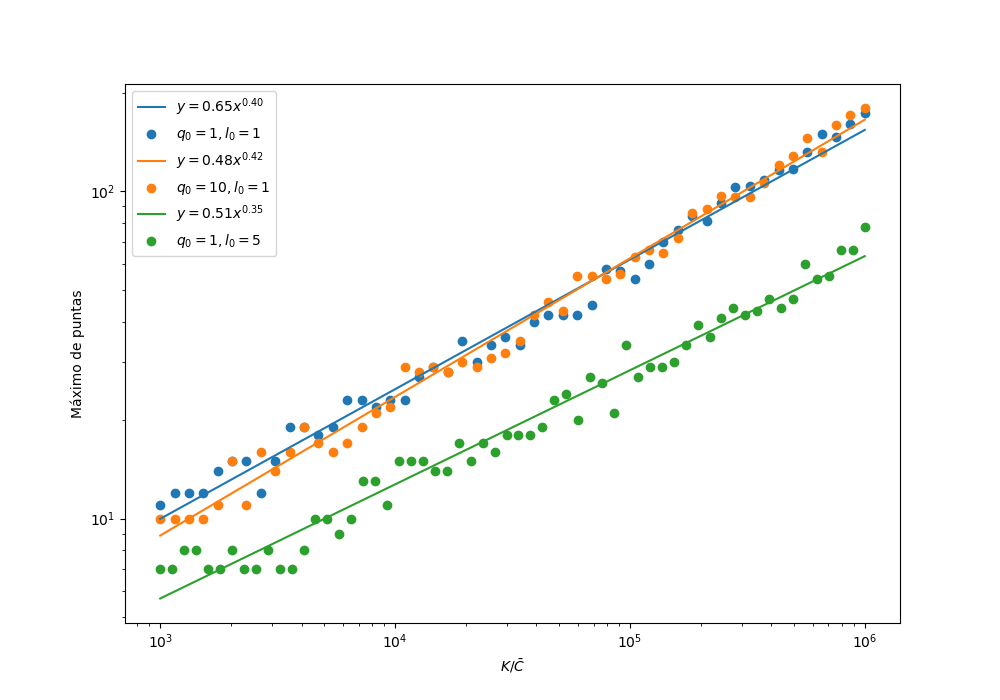
\includegraphics[width=0.8\textwidth]{graficos_inst/max_vs_KC.png}
    \caption{Tamaño máximo alcanzado en función de $K/\bar{C}$.}
    \label{fig:max_vs_KC}
\end{figure}

El tamaño máximo del sistema escala como potencia de esta razón, con exponente $\simeq 0.4$. El coeficiente multiplicativo no parece depender del flujo $q_0$, pero sí de $l_0$.

\subsection{Fase de exploración y Cambio de fase}

Veamos la evolución del árbol durante la fase de crecimiento, en particular el tamaño (Fig. \ref{fig:l_vs_tiempo_princ} y Fig. \ref{fig:N_vs_tiempo_princ})

\begin{figure}[h!]
\begin{minipage}{0.5\textwidth}
    \centering
    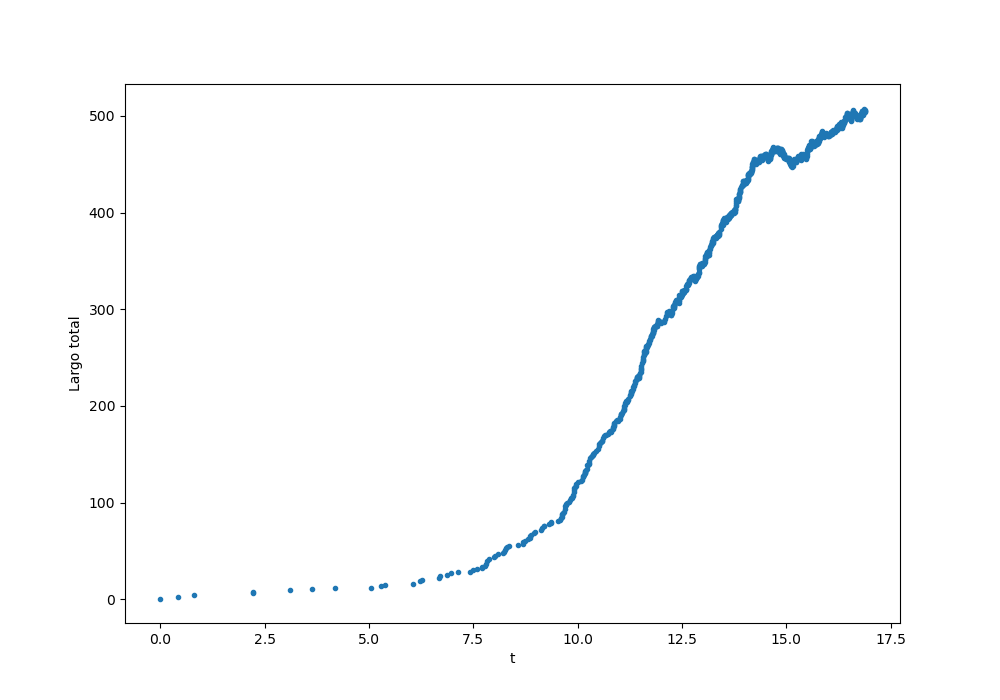
\includegraphics[width=\textwidth]{graficos_inst/largo_vs_tiempo_principio.png}
    \caption[]{Evolución del largo total}
    \label{fig:l_vs_tiempo_princ}
\end{minipage} 
\begin{minipage}{0.5\textwidth}
    \centering
    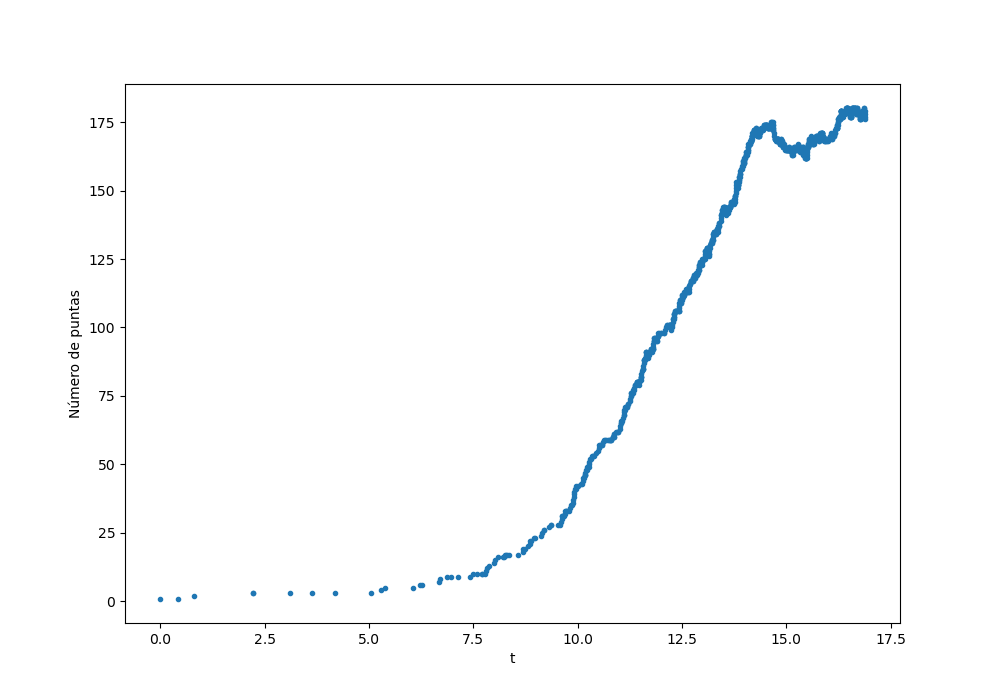
\includegraphics[width=\textwidth]{graficos_inst/N_vs_tiempo_principio.png}
    \caption[]{Evolución de las puntas}
    \label{fig:N_vs_tiempo_princ}
\end{minipage}   
\end{figure}

Ambos valores crecen (casi) exponencialmente, hasta alcanzar un máximo y luego entrar en la fase estacionaria.

Sería interesante estudiar cómo varía el cambio de fase con los diferentes parámetros, y relacionarlo al tamaño máximo, ya que estos ocurren básicamente al mismo tiempo.
\section{Ley de Murray}

Uno de los objetivos es ver que la ley de Murray va a aparecer por si sola en el sistema, sin ser impuesta. Pero esto resulta ser evidente (y en realidad sí es impuesta, sólo indirectamente):

Sea $C_0$ un ducto padre y $C_1$, $C_2$ sus "hijos". El ducto $C_1$ es atravesado por $Q_1$, y $C_2$ por $Q_2$, por lo que $C_0$ es atravesado por $Q_0 = Q_1 + Q_2$. Entonces, las conductancias óptimas son:

$$ C_i^* = \frac{Q_i^{4/3} K}{S^2 l_i} \quad i\in\{0,1,2\} $$

Con $ S = \sum_{<ij>}Q_{ij}^{2/3}l_{ij} $

Luego, podemos encontrar el radio óptimo:

$$ r_i = \left( C_i^* l_i \frac{8 \mu}{\pi} \right)^{1/4} = \frac{Q_i^{1/3}}{S^{1/2}}\left(\frac{8K\mu}{\pi}\right)^{1/4}$$

Y encontramos, efectivamente:

\begin{align*}
    r_1^3 + r_2^3 & = \left(\frac{Q_1 + Q_2}{S^{3/2}}\right)\left(\frac{8K\mu}{\pi}\right)^{3/4} \\
    & = r_0^3
\end{align*}

¡La ley se cumple directamente!

Para estudiarlo en el modelo, vemos como evoluciona el valor promedio de $\frac{r_0^3}{r_1^3+r_2^3}$.

\begin{figure}[h!]
    \centering
    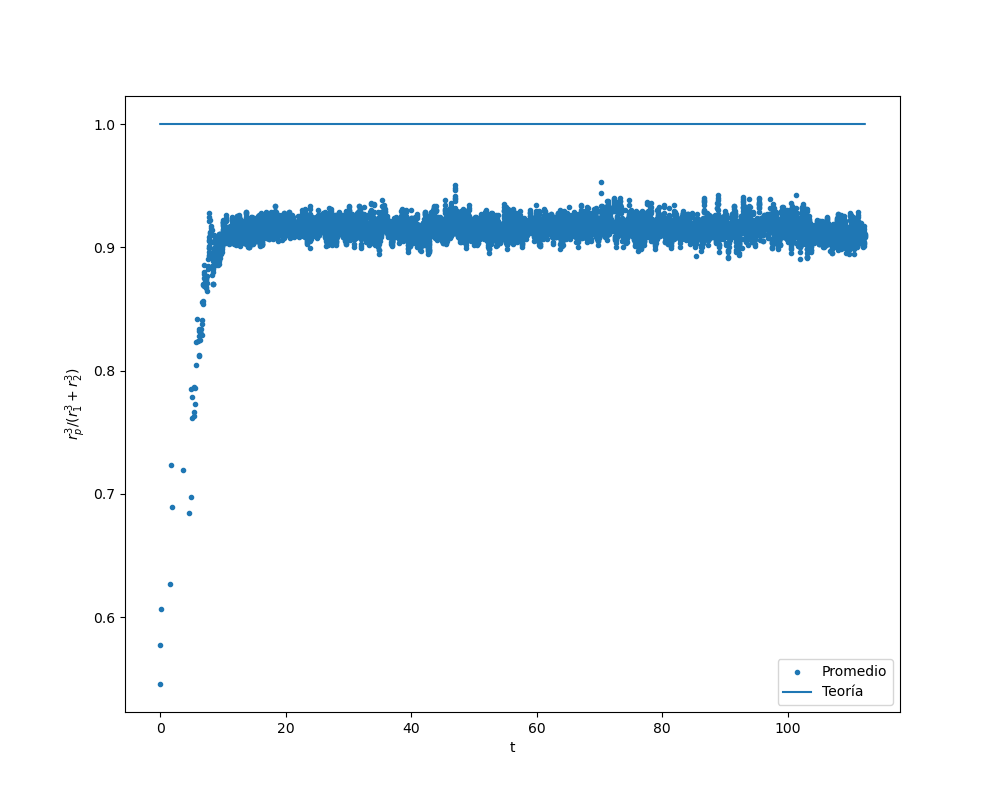
\includegraphics[width=0.8\textwidth]{graficos_inst/murray_feo.png}
    \caption{Ley de Murray con el flujo promediado sobre 10 iteraciones.}
    \label{fig:murray_feo}
\end{figure}

En la simulación, existe un leve offset y ruido, pero la ley parece cumplirse. Este offset se debe al tiempo que requieren en adaptarse los flujos promedios, siendo que las conductancias (los radios), se adaptan instantáneamente de forma "errónea". Esto es más evidente al principio, cuando el sistema es joven y pequeño (una cantidad baja de bifurcaciones para promediar), por lo que parece converger hacia un valor.

En efecto, cuando el padre se bifurca, su flujo promedio es básicamente $q_0$, ya que era una punta. Como este se promedia sobre varias iteraciones (acá 10), tenemos durante un cierto tiempo:

$$ q_0 \simeq  \langle Q_{0}(t)\rangle_T < \langle Q_{1}(t)\rangle_T + \langle Q_{2}(t)\rangle_T \simeq 2q_0$$

Como los cubos de los radios son proporcionales a los flujos: $r_0^3 < r_1^3 + r_2^3$ Es lo que vemos en el gráfico. Para un promedio sobre 10 iteraciones, la razón $\frac{r_0^3}{r_1^3+r_2^3}$ está cerca de $0.9$. Mientras menos iteraciones se promedien, más se acerca a 1. En efecto, como es esperado por la demostración anterior, para un flujo instantáneo (que no se promedia) vemos (Fig. \ref{fig:murray_lindo}):

\begin{figure}[h!]
    \centering
    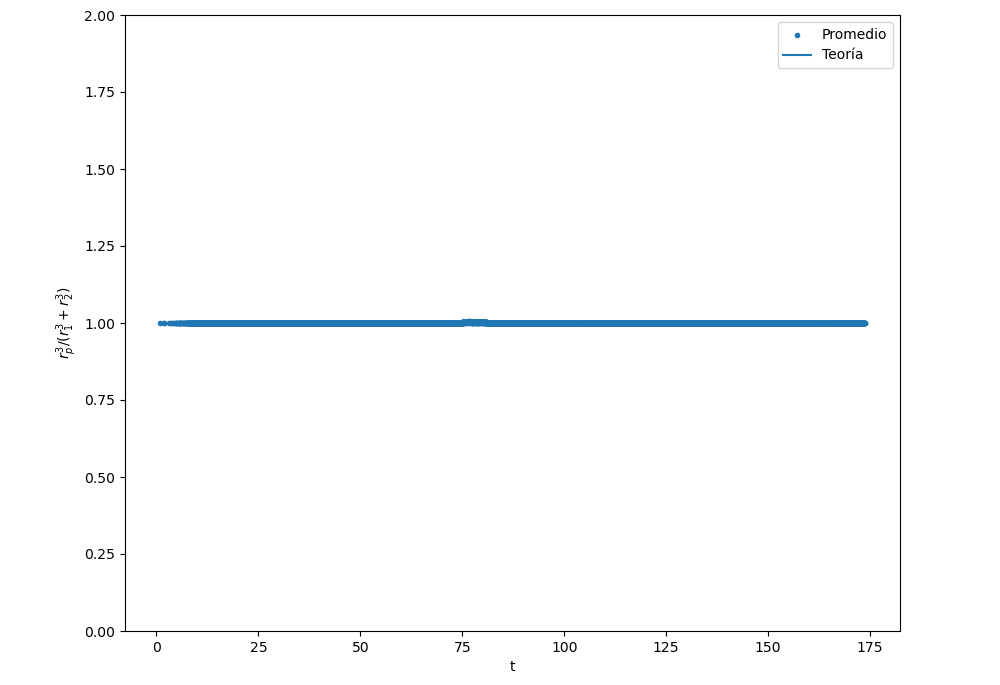
\includegraphics[width=0.8\textwidth]{graficos_inst/murray_lindo.png}
    \caption{Ley de Murray con flujo instantáneo.}
    \label{fig:murray_lindo}
\end{figure}
\newpage
\section{Topología}

Para estudiar características topológicas del sistema, lo generamos con $K$ muy grande, para así tener un estado estacionario grande igualmente.

Partimos viendo el largo promedio en función de la generación (Fig. \ref{fig:largo_vs_gen}). Cada color representa un momento diferente del sistema.

\begin{figure}[h!]
    \centering
    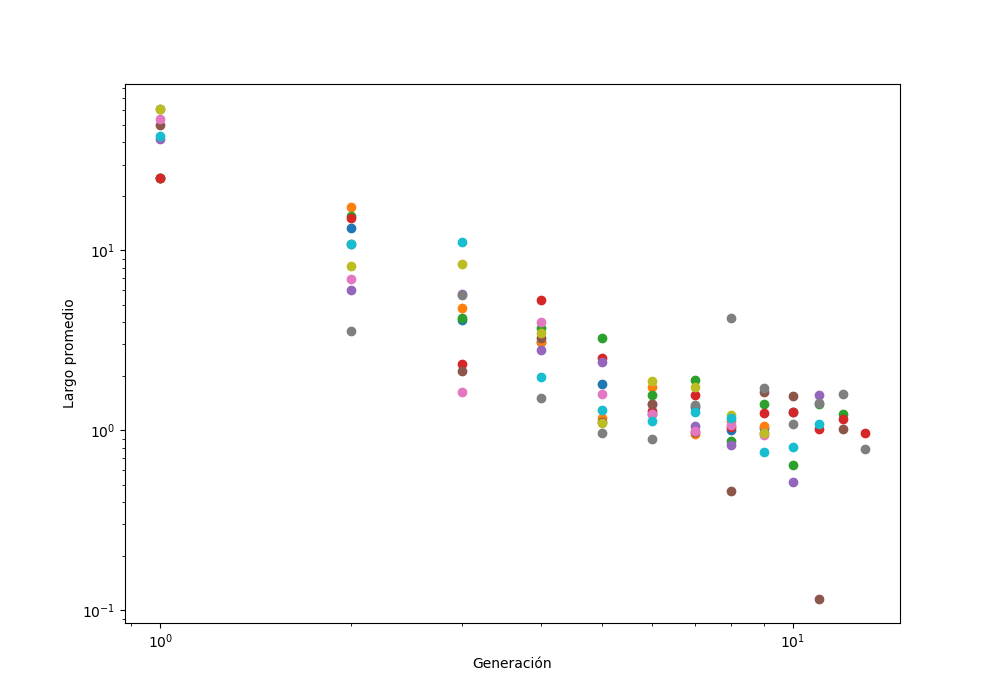
\includegraphics[width=0.8\textwidth]{graficos_inst/largo_vs_gen.png}
    \caption{Largo promedio por generación.}
    \label{fig:largo_vs_gen}
\end{figure}

Vemos que el largo promedio decae con la generación, lo que es esperable. Algo interesante de estudiar sería cómo varía este decaimiento en el tiempo, y si converge hacia algo estable, pero no pareciera ser así: Los diferentes estados del sistema fueron tomados en estado estacionario, separados de 100 iteraciones y aún así existe una gran variación.

Veamos luego lo que ocurre con los radios en esta misma simulación (Fig. \ref{fig:radio_vs_gen}):

\begin{figure}[h!]
    \centering
    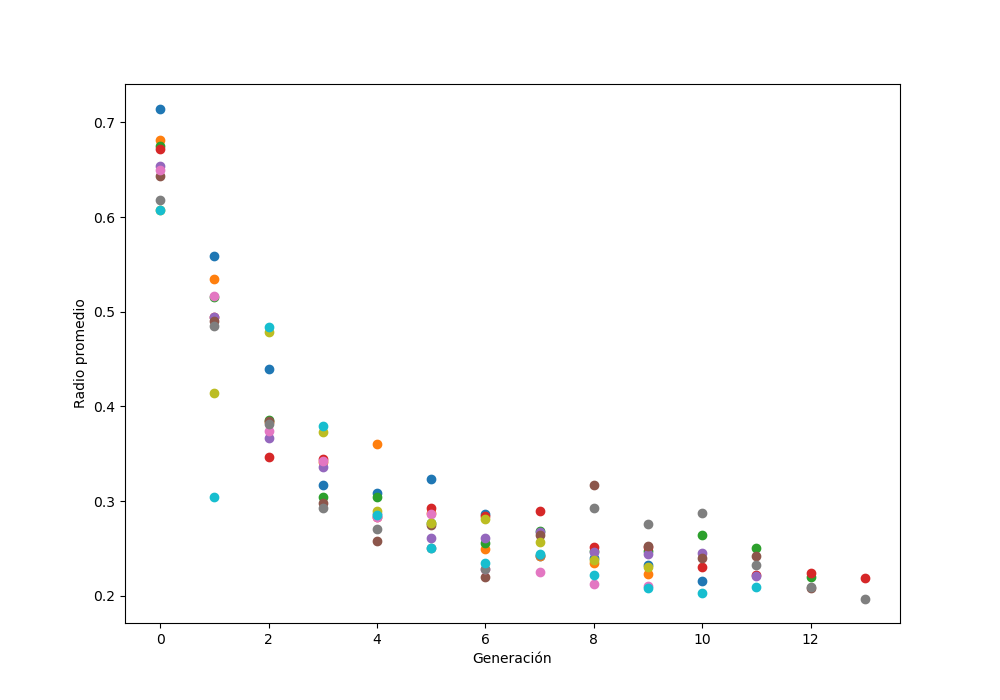
\includegraphics[width=0.8\textwidth]{graficos_inst/radio_vs_gen.png}
    \caption{Radio promedio por generación.}
    \label{fig:radio_vs_gen}
\end{figure}

El decaimiento exponencial es mucho más claro.

\textbf{Limitaciones}: En cuanto a otras características, como la probabilidad de terminación, no pude encontrar nada significativo por la rápida variación y pocas generaciones del sistema. Para encontrar algo, tal vez se debería generar un sistema de mucho mayor tamaño.

\section{Modelo paulatino}

Para este modelo final, y más realista, el sistema puede adaptarse con una velocidad máxima.

Definimos $v_0$, la velocidad de propagación de los ductos. En un ducto de material (área) constante, tenemos la relación:

\begin{align*}
    & 2\pi r_{ij}(t) l_{ij}(t) = A \\
    \implies & \frac{d r_{ij}}{dt} l_{ij} + \frac{d l_{ij}}{dt} r_{ij} = 0 \\
    \implies & \frac{d r_{ij}}{dt} = - v_0 \frac{r_{ij}}{l_{ij}}
\end{align*}

Como $C_{ij} = \frac{\pi r_{ij}^4}{8\mu l_{ij}}$, entonces:

\begin{align*}
    \frac{d C_{ij}}{dt} & = \frac{\pi}{8\mu} \frac{4 \dot{r_{ij}}r_{ij}^{3} l_{ij} - \dot{l_{ij}}r_{ij}^{4}}{l_{ij}^{2}}\\
    & = \frac{\pi}{8\mu} \frac{- 4v_0 r_{ij}^{4} - v_0 r_{ij}^{4}}{l_{ij}^{2}} \\
    & = \frac{\pi}{8\mu} \frac{- 5v_0 r_{ij}^{4}}{l_{ij}^{2}} \\
    & = \frac{-5 v_0}{l_{ij}} C_{ij}
\end{align*}

Con estas velocidades, podemos hacer que el crecimiento del sistema, y la adaptación frente a este, sean paulatinos.

\textbf{Desafío pendiente}: La optimización también debería hacerse paulatinamente, de forma que un sistema estacionario tienda hacia las conductancias óptimas. Pero el sistema va cambiando constantemente, por lo que implementar esto correctamente requiere mayor desarrollo.

\section{Trabajo futuro}

Todavía se puede ahondar mucho en estas y otras características del modelo que no alcancé por falta de tiempo. También es necesario aumentar la cantidad de datos y promediar sobre diferentes simulaciones, para tener valores más exactos.
Un problema con esto es la gran variabilidad de las simulaciones, y el manejo de grandes cantidades de datos (que me superó).

\end{document}